\providecommand{\main}{..}
\documentclass[\main/notes.tex]{subfiles}

\begin{document}
	\setcounter{chapter}{13}
	\chapter{Databases}
		\section{Introduction}
			\begin{definition}{Database}
				A collection of related, logically consisten, data used by the application programs in an organization.
			\end{definition}
			\subsection{Advantages of Databases}
				\begin{indentparagraph}
					\begin{description}
						\item[Less redundancy] Information is stored in one file, rather than repeated in many places.
						\item[Inconsistency avoidance] When information is updated, in a flat strcuture, the information needed to be updated in multiple places. If a place is not updated, then this information is inconsistent with the rest. Databases avoid this, by having a single location.
						\item[Efficiency] Information stored in fewer locations, so faster to access
						\item[Data integrity] Easier to ensure data is accurate, as fewer locations
						\item[Confidentiality] Easier to ensure security, and therefore confidentiality, as data is in a central location.
					\end{description}
				\end{indentparagraph}
			\subsection{Database Management Systems}
				\begin{definition}{Database Management System (DBMS)}
					Defines, creates and maintains a database. Also allows controlled access to data in the database. Has five components: \concept{hardware}, \concept{software, \concept{data}}, \concept{users}, and \concept{procedures}.
					\begin{center}
						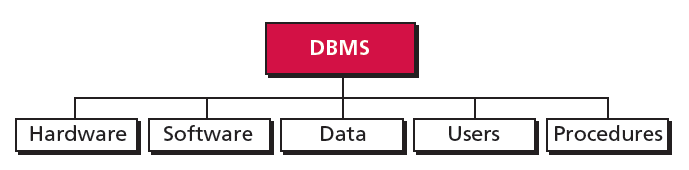
\includegraphics[width=0.6\textwidth]{\main/images/unit14/dbms_components.png}
					\end{center}
				\end{definition}
				\pagebreak
				\begin{description}
					\item[Hardware] The physical computer system that allows access to the data
					\item[Software] The program that allows users to access, maintain, and update data. Also controls which user can access which parts of the data in the database
					\item[Data] Stored physically on storage devices. A separate entity from the software that accesses it. This separation allows the organization to change the software without needing the change the physical data, or the way it is stored.
					\item[Users] Can be divided into two categories: \concept{end users}, and \concept{application} programs.
						\begin{description}
							\item[End users] Humans who access the database directly to get information. Two types: \concept{database administrators (DBAs)}, and \concept{normal users}. DBAs have the maximum level of priveleges, and control other users and their access to the DBMS. A normal user can only use part of the database, and has limited access.
							\item[Application programs] Applications that access and process data from a DBMS.
						\end{description}
					\item[Procedures] A clearly defined set of procedures or rules that must be followed by users of the database.
				\end{description}

		\section{Database Architecture}
			A three-level architecture is used for a DBMS: \concept{internal}, \concept{conceptual}, and \concept{external}.
			\begin{center}
				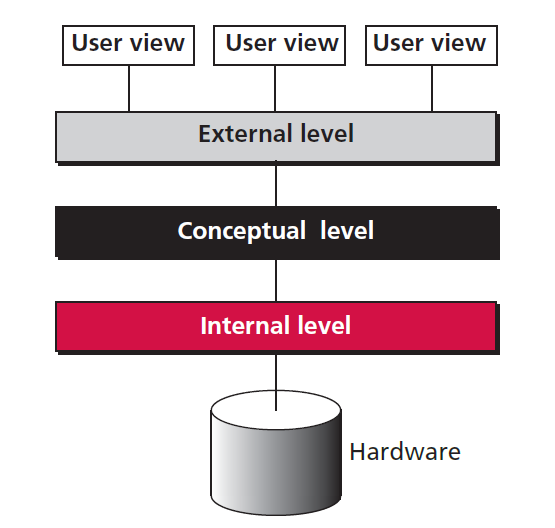
\includegraphics[width=0.35\textwidth]{\main/images/unit14/database_architecture.png}
			\end{center}
			\begin{description}
				\item[Internal Level] Determines where the data is actually stored on storage devices. Low-level access methods, and how bytes are transferred to and from storage devices.
				\item[Conceptual Level] Defines the logial view of the data. The data movel is defined on this level, and the main functions of the DBMS (eg. queries) are on this level.
				\item[External Level] Interacts directly with the user. Changes the data coming from the conceptual level to a format and view that is familiar to users.
			\end{description}

		\pagebreak
		\section{Database Models}
			\begin{definition}{Database Model}
				Defines the logical design of data. Also describes the relationships between different parts of the data.
			\end{definition}
			\subsection{Hierarchical Database Model}
				\begin{definition}{Hierarchical Database Model}
					An obsolete model.

					Data is organised as an inverted tree. Each entity has only one parent, but can have several children. At the top of the hierarchy, there is one entiry, called the \concept{root}.

					\begin{center}
						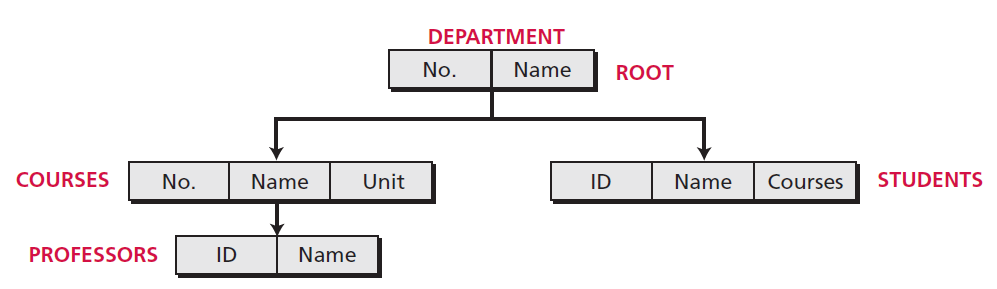
\includegraphics[width=0.8\textwidth]{\main/images/unit14/hierarchical_model.png}
					\end{center}
				\end{definition}
			\subsection{Network Database Model}
				\begin{definition}{Network Database Model}
					An obsolete model.

					Entities are organised in a graph, where some entities can be accessed through several paths. There is no hierarchy.

					\begin{center}
						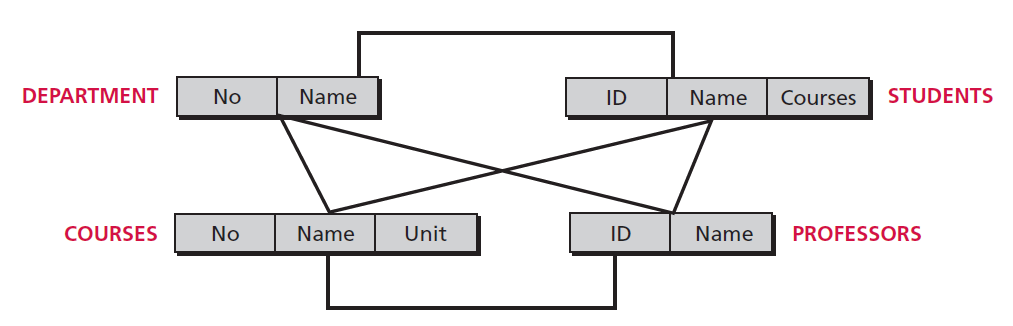
\includegraphics[width=0.8\textwidth]{\main/images/unit14/network_model.png}
					\end{center}
				\end{definition}
			\pagebreak
			\subsection{Relational Database Model}
				\begin{definition}{Relational Database Model}
					Data is organised in two-dimensional tables called \concept{relations}. No hierarchical or network structure is impoed on the data. The tables are related to each other.

					\begin{center}
						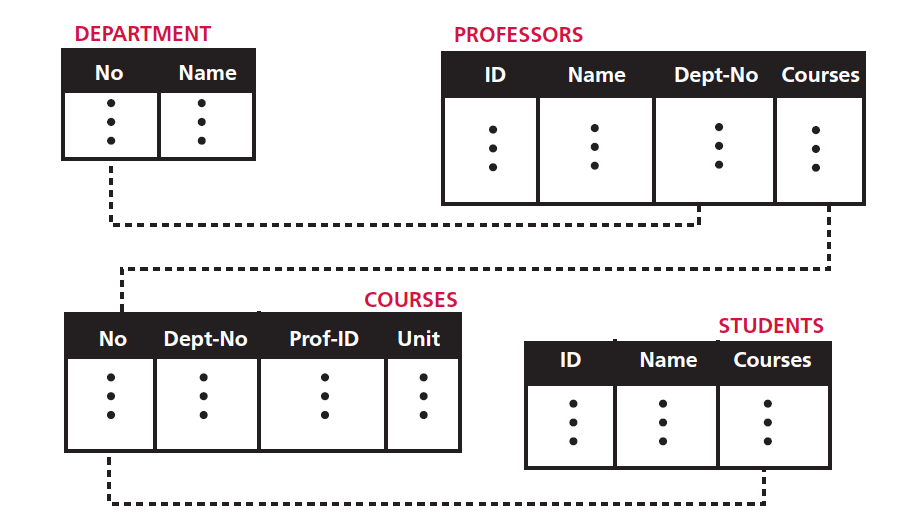
\includegraphics[width=0.8\textwidth]{\main/images/unit14/relational_model.png}
					\end{center}

					Two models are derived from this model: the distributed model, and the object-oriented model.
				\end{definition}

		\section{Relational Database Model}
				Data is represented as a set of \concept{relations}.
				\begin{definition}{Relation}
					Appears as a two-dimensional table. Has the following features:
					\begin{indentparagraph}
						\begin{description}
							\item[Name] The name of the table/relation. Should be unique among other relations.
							\item[Attributes] The columns in the relation. Gives meaning to the data stored under the column heading. Must be unique in each table. The number of attributes is called the \concept{degree} of the relation. Not stored in the database -- the conceptual level uses the atributes to give meaning to each column.
							\item[Tuples] The rows in a relation. Defines a collection of attribute values. The total number of rows in a relation is called the \concept{cardinality}. The cardinality changes when tuples are added or deleted -- the database is dynamic.
						\end{description}
					\end{indentparagraph}
					\begin{center}
						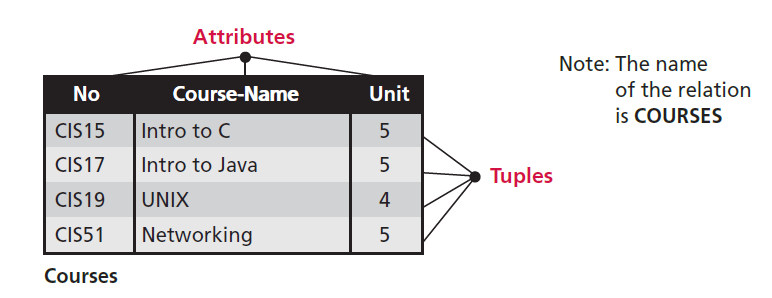
\includegraphics[width=0.6\textwidth]{\main/images/unit14/relation_example.png}
					\end{center}
				\end{definition}
			\subsection{Operations on Relations}
				Operations can be defined to create new relations based on existing ones.
				\begin{definition}{Structured Query Language (SQL)}
					Language standardised for use on relational databases. Declarative tather than procedural. First implemented by Oracle Corporation in 1979.
				\end{definition}
				\begin{center}
					\begin{tblr}{colspec={ccl}}
						Operation & Type & Description\\
						\midrule
						Insert & Unary & Inserts a new tuple into the relation\\
						Delete & Unary & Deletes a tuple from the relation\\
						Update & Unary & Changes the values of some attributes of a tuple\\
						Select & Unary & Create another relation (same attributes, less tuples)\\
						Project & Unary & Create another relation (same tuples, less attributes)\\
						Join & Binary & Combine relations based on common attributes\\
						Union & Binary & Combine two relations that have the same attributes \nl (include if in either)\\
						Intersection & Binary & Take two relations that have the same attributes \nl (include only if in both)\\
						Difference & Binary & Subtract a relation from another \nl (return the tuples in first but not second)
					\end{tblr}
				\end{center}
				\subsubsection{Unary Operations}
					\begin{definition}{Insert Operation}
						Inserts a new tuple into the relation.
						\begin{center}
							\texttt{insert into RELATION-NAME values (\ldots, \ldots, \ldots)}
						\end{center}
						\texttt{values} defines all the attribute values for the corresponding tuple.
					\end{definition}
					\begin{definition}{Delete Operation}
						Deletes a tuple based on given critera.
						\begin{center}
							\texttt{delete from RELATION-NAME where criteria}
						\end{center}
					\end{definition}
					\begin{definition}{Update Operation}
						Changes the value of some attibutes of a tuple.
						\begin{center}
							\begin{tabular}{c}
								\begin{lstlisting}
	update RELATION-NAME
	set attribute1 = value1, attribute2 = value2
	where criteria
								\end{lstlisting}
							\end{tabular}
						\end{center}
					\end{definition}
					\begin{definition}{Select Operation}
						Creates another relation, where the tuples (rows) in the relation are a subset of the tuples in the original relation. Fewer tuples than the original relation, same number of attributes.
						\begin{center}
							\texttt{select * from RELATION-NAME where critera}
						\end{center}
						\texttt{*} is used to show that all attributes are chosen.
					\end{definition}
					\begin{definition}{Project Operation}
						Creates another relation, where the attributes (columns) are a subset of the attributes in the original relation. Fewer attributes than the original relation, same number of tuples.
						\begin{center}
							\texttt{select attribute\_list from RELATION-NAME}
						\end{center}
					\end{definition}
				\subsubsection{Binary Operations}
					\begin{definition}{Join Operation}
						Combines two relations based on common attributes.
						\begin{center}
							\begin{tabular}{c}
								\begin{lstlisting}
	select attribute_list
	from RELATION1, RELATION2
	where criteria
								\end{lstlisting}
							\end{tabular}
						\end{center}
					\end{definition}
					\begin{definition}{Union Operation}
						\emph{Both relations must have the same attributes}. Creates a new relation in which each tuple is either in the first relation, in the second, or both.
						\begin{center}
							\begin{tabular}{c}
								\begin{lstlisting}
	select * from RELATION1
	union
	select * from RELATION2
								\end{lstlisting}
							\end{tabular}
						\end{center}
					\end{definition}
					\begin{definition}{Intersection Operation}
						\emph{Both relations must have the same attributes}. Creates a new relation in which each tuple is in both the first relation and the second relation.
						\begin{center}
							\begin{tabular}{c}
								\begin{lstlisting}
	select * from RELATION1
	intersection
	select * from RELATION2
								\end{lstlisting}
							\end{tabular}
						\end{center}
					\end{definition}
					\pagebreak
					\begin{definition}{Difference Operation}
						\emph{Both relations must have the same attributes}. Results in a relation that contains the tuples that are in the first relation, but not the second.
						\begin{center}
							\begin{tabular}{c}
								\begin{lstlisting}
	select * from RELATION1
	minus
	select * from RELATION2
								\end{lstlisting}
							\end{tabular}
						\end{center}
					\end{definition}

	\ifSubfilesClassLoaded{%
		\vbox{\rulechapterend}}{\vspace*{\parskip}\rulebookend}
\end{document}